%% LyX 2.1.2 created this file.  For more info, see http://www.lyx.org/.
%% Do not edit unless you really know what you are doing.
\documentclass[english]{article}
\usepackage[T1]{fontenc}
\usepackage[latin9]{inputenc}
\usepackage{amsmath}
\usepackage{graphicx}

\makeatletter

%%%%%%%%%%%%%%%%%%%%%%%%%%%%%% LyX specific LaTeX commands.
%% Because html converters don't know tabularnewline
\providecommand{\tabularnewline}{\\}

\@ifundefined{showcaptionsetup}{}{%
 \PassOptionsToPackage{caption=false}{subfig}}
\usepackage{subfig}
\makeatother

\usepackage{babel}
\begin{document}

\section{Elastic influence testing and implementation}


\subsection{Two nearby parallel fractures \label{sub:Two-nearby-parallel}}

\begin{figure*}[t]
\centering\subfloat{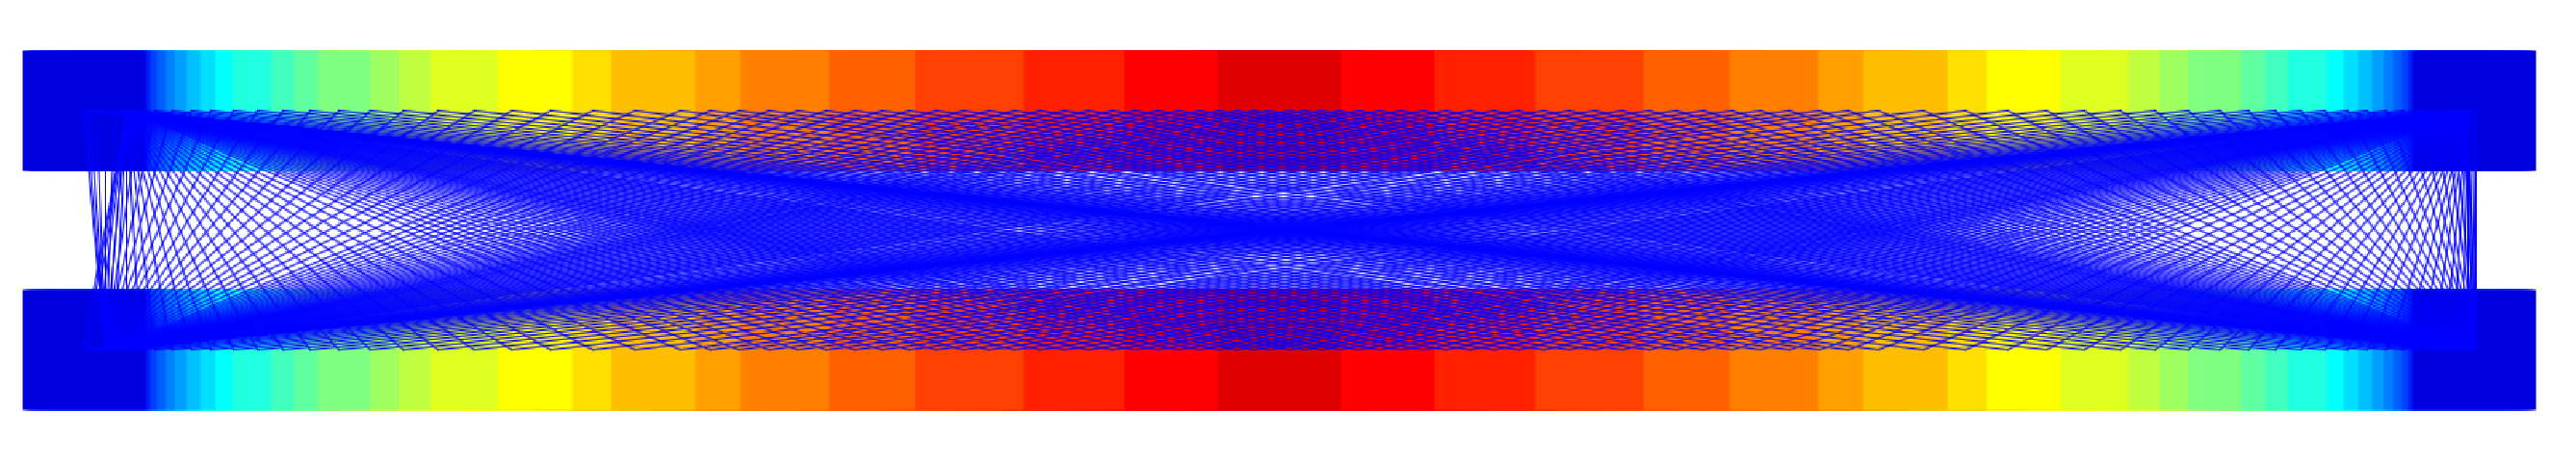
\includegraphics[scale=0.1]{two_close_fractures}}

\protect\caption{Placeholder graphic. Two close parallel fractures.}


\label{two_close_paraller}
\end{figure*}


As the first test for pseudo elastic influence procedure, lets consider
a relatively simple case where two fractures are placed parallel to
each other, and aligned as if there were mirror images of each other.
This is similar to the case described by Bunger \cite{Bunger}, except
for the fact that only two fractures are presents, hence$\sigma_{l}$
value should be half of the expected value form relation (\ref{sigma_close}).
Given that the both fracture height and spacing are set to $1$, one
should expect to for our elastic scheme to produce a result that follows:

\begin{equation}
\sigma_{l}(x)=\frac{3}{16}p_{net}(x)\label{eq:expected_two_fracures_elasticity}
\end{equation}


From the above one can work out the value of $g$ in (\ref{sigma_formula}),
as this is the only unknown parameter. The approximate value proposed
here is:

\begin{equation}
g=0.1413\label{eq:g_value}
\end{equation}


This value of $g$ allows the pseudo elastic influence used here to
match the value one would expect form Bunger scheme \cite{Bunger},
at the crack inlet $x=0$. The comparison of the two schemes is shown
on Figure (\ref{two_close_paraller_graph}). However, Bungers method
\cite{Bunger} was derived for very long fractures, thous the effect
of tip region where width rapidly detergents to zero, and consequently
the region with no opened fracture that follows, was not included,
the whole fracture aperture was essential treated as flat surface.
Therefore to find matching value of $g$, approximation was made for
a case where fracture half length $L=100$. This produces a nearly
perfect match as $L$ is indeed much larger than the spacing (accuracy
grater than internal relative tolerance set to $10^{-3}$, see Section
below \ref{sub:Approximation-tolerances,-and}). In cases when shorter
fractures are considered, namely $L=10$ and $L=1$, greater discrepancy
can be observed especially for $x>0.9$ where a switch form underestimation
to overestimation of $\sigma_{l}$ value can be observed. When fracture
length is lesser than the distance, as for example $L=\frac{1}{4}$,
shape of $\sigma_{l}$ changes to a constant line, which represents
switch to the far field approximation (\ref{sigma_far}).

\begin{figure*}[t]
\centering\subfloat[Values of $\sigma_{l}$ for different half fracture lengths.]{

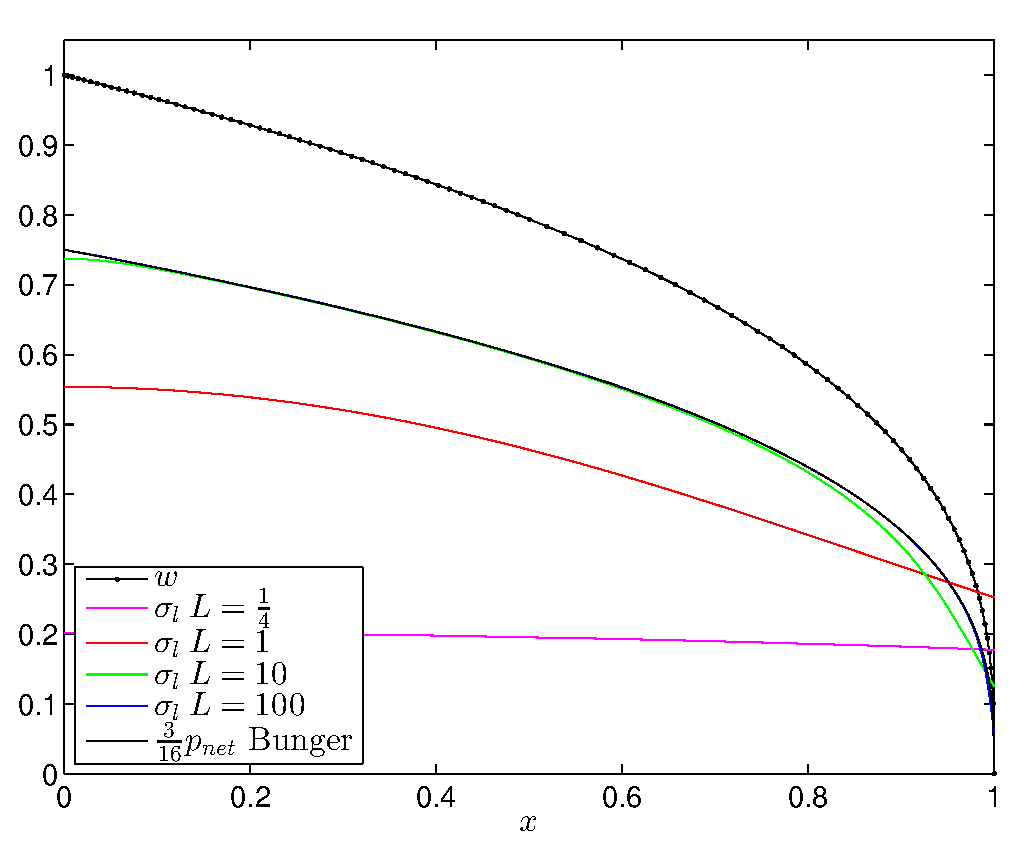
\includegraphics[scale=0.6]{elasticity_two_fracures}

}

\subfloat[Relative discrepancies of $\sigma_{l}$ from close approximation \ref{eq:expected_two_fracures_elasticity}
for different half fracture lengths.]{

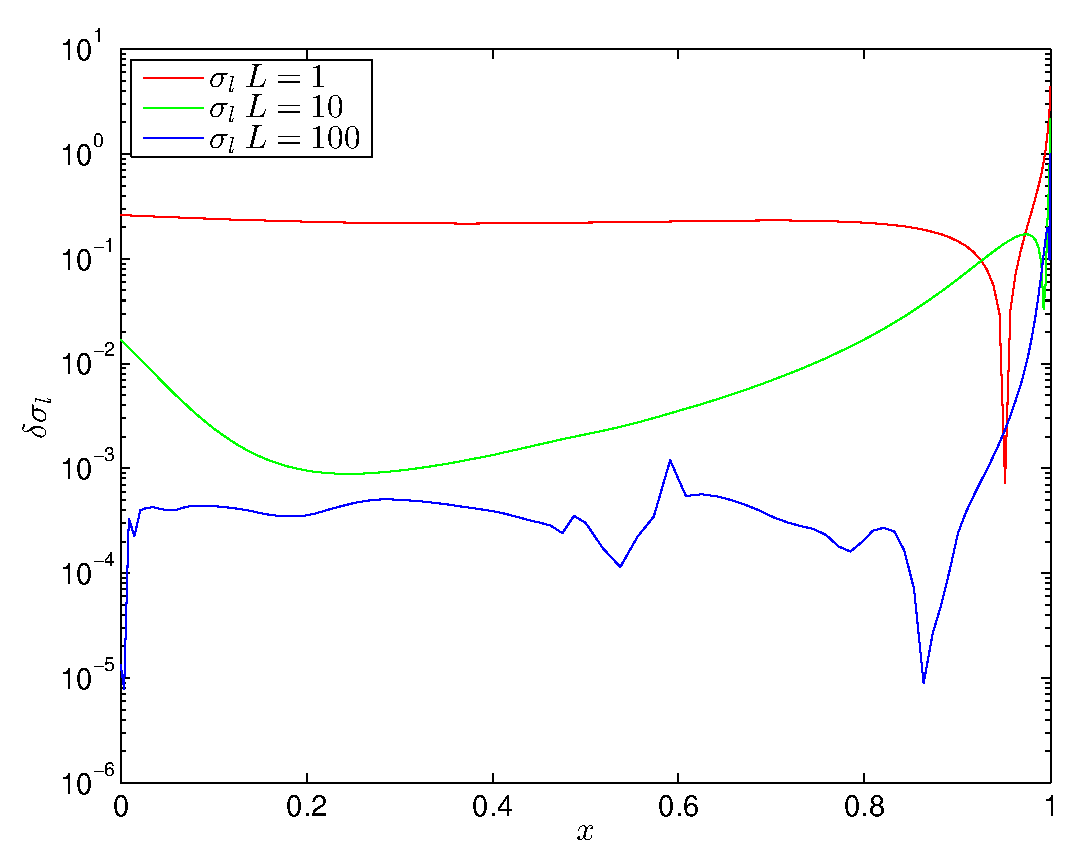
\includegraphics[scale=0.6]{elasticity_two_fracures_reltol}

}

\protect\caption{Elasticity effect of two close parallel fractures. Values of $\sigma_{l}$
depending on the half fracture length.}


\label{two_close_paraller_graph}
\end{figure*}


\clearpage


\subsection{Two fractures from common junction \label{sub:Two-fractures-from}}

Here the calculation of $\sigma_{l}$ for two connected fractures
will be tested. Suppose that there are two fractures originating form
the same point (wellbore), that for this particular test scenario
are placed at some angle $\alpha$ between them, as shown on Figure
(\ref{sigma_on_connected_fractures}). This setting gives a good opportunity
to test the effect of distance term $\frac{1}{min(d^{3},1)}$ in (\ref{sigma_formula}).
If strict $\frac{1}{d^{3}}$ was to be used a singularity would appear
when $x\rightarrow0$. This would be disastrous. Furthermore note
that the single fracture formulation already effectively normalized
\ref{elasticity} fracture height to $1$, hence when $d=1$ the term
$\frac{1}{d^{3}}$, which is valid in three dimensions, could be switched
to $\frac{1}{d^{2}}$, as the problem now is closer.

Should this result be repeated in other computations ? Lets remind
ourselves that vector $\hat{\sigma}$ is computed (\ref{sigma_formula})
from the fracture propagation axis $x$, that is in the middle of
the fracture, but not from the fracture surface. Under most conditions
$w<<L$, thous the slight deviation form location on crack surface
and middle would not matter, but here as these fractures are interconnected
a small overlapping region appears (Figure (\ref{sigma_on_connected_fractures})).
Properly modeling this region is beyond current problem formulation,
thous some approximation will be used here. Here a change of distance
dependence term in$\sigma$ to will be considered $\frac{1}{max(d^{3},1)}$
. (NOTE fracture height$h$ is already normalized to 1 ) While the
theoretical motivation behind this change can be questioned, it is
a very simple and practical way to handle the problem of overlapping
region. Naturally one could follow more accurate and complex solutions
such as one used by\cite{Kresse2}. (not sure if that one actually
is concerned with this problem). 

TBC

\begin{figure*}[t]
\centering

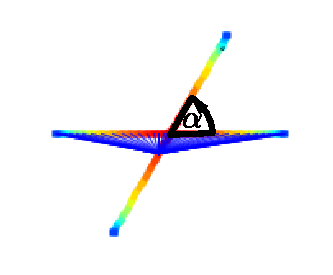
\includegraphics[scale=1.5]{ang_1}

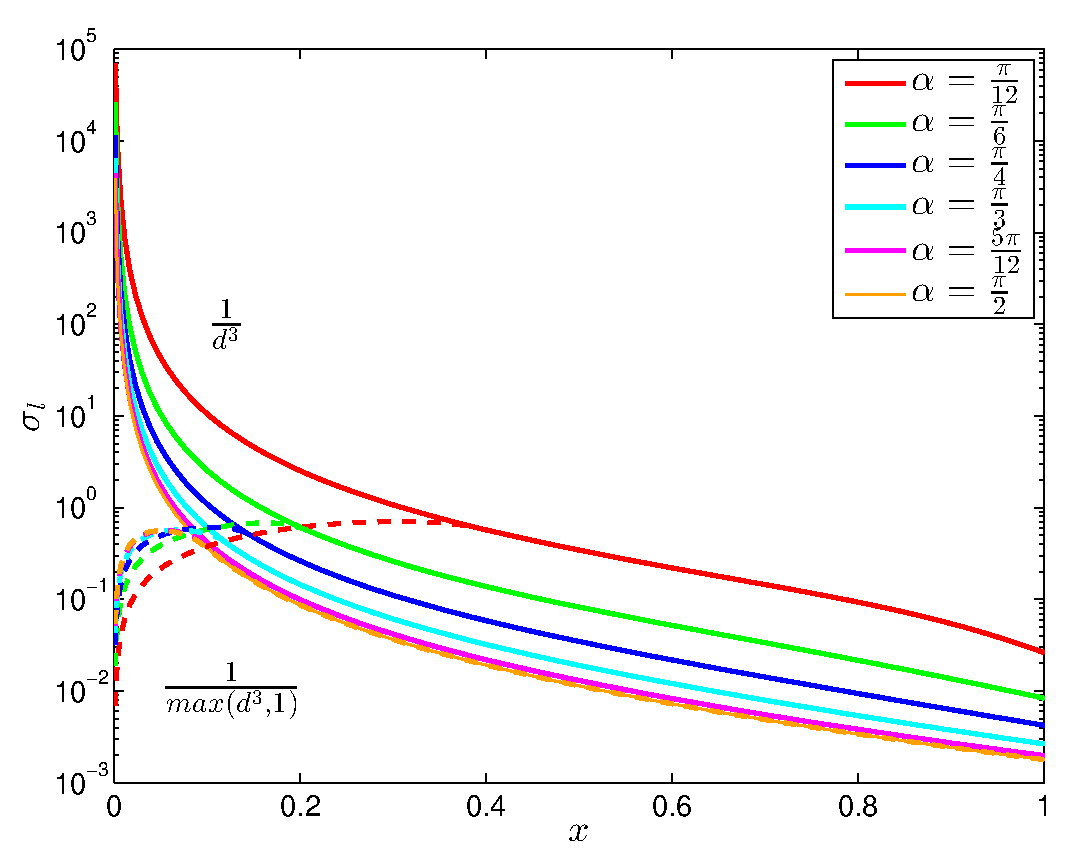
\includegraphics[scale=0.6]{angle1}

\centering

\protect\caption{Value of $\sigma_{l}$ for two connected fractures. \ref{sigma_formula}}


\label{sigma_on_connected_fractures}
\end{figure*}


\clearpage


\subsection{Approximation tolerances, and fast square root \label{sub:Approximation-tolerances,-and}}

The recursive method for approximation of (\ref{sigma_formula}) described
in Section \ref{sec:Method-for-elasticity} uses tolerance thresholds
$\sigma_{l}^{reltol}$ and $\sigma_{l}^{abstol}$ to decide when to
stop recursion (\ref{eq:elasticity_recursive_condition}). The previously
considered case of two close parallel fractures, as shown on Figure
\ref{two_close_paraller} can be used to measure the effects of different
tolerances on the final value of $\sigma_{l}$. The spacing is set
to$1$ while $L=100$ to increase number the divisions needed to achieve
desired accuracies. .Results of such measurements for three pairs
of tolerance values are shown on Figure \ref{sigma_tols}. The baseline
comparison is a result obtained with $\sigma_{l}^{reltol}=\sigma_{l}^{abstol}=10^{-12}$.
Increasing the tolerances to $\sigma_{l}^{reltol}=10^{-4},\sigma_{l}^{reltol}=10^{-8}$
reduces the accuracy but to a level comparable with $\sigma_{l}^{reltol}=10^{-3},\sigma_{l}^{reltol}=10^{-6}$
when considering the proximity of end interval points $x=0$ and $x=1$.
However further increase to $\sigma_{l}^{reltol}=10^{-2},\sigma_{l}^{reltol}=10^{-4}$
results in unsafe relative values of $\delta\sigma_{l}$, that exceed
$10^{-2}$, thous less strict tolerances should not be used.

The reason for seeking optimal values $\sigma_{l}^{reltol}$ and $\sigma_{l}^{abstol}$,
is that the lower the tolerances are, the more recursive steps are
needed to find (\ref{sigma_formula}), and thous more time is consumed.
Since the general accuracies of this multifracturing model are unlikely
to be greater than $10^{-5}$ (see Section \ref{sub:Comparison-of-ODE}
), using methods of higher accuracies will be somehow a waste of resources.
Meanwhile finding other means off speeding up this elasticity calculation
may prove to be very beneficial for overall performance.

An additional improvement can be achieved by tweaking the inverse
square root present in (\ref{sigma_formula}): 
\begin{equation}
\frac{1}{d^{3}}\xrightarrow{requires}\frac{1}{\sqrt{x}^{3}}\label{eq:inverse_sqrt_is_neede}
\end{equation}


Interestingly so far the majority of this work could be implemented
only as numerical additions, subtractions, multiplications and divisions.
The whole pseudo-elasticity scheme \ref{sec:Method-for-elasticity}
does not require any more complex mathematical functions, except for
$\sqrt{x}$ required to calculate the distance $d$. The simplest
approach is to use the existing native sqrt() function, available
in all programing languages. This function however has one significant
disadvantage: its accuracy is extremely high, while the time cost
can be in hundreds of CPU cycles. Unfortunately, $\sqrt{x}$ will
be used a lot of times in this multifracturing problem, but there
are other great works where the issue of native sqrt() performance
was fixed. 

A number of 3D graphics problems requires massive repeated calculations
of surface normals, which can be speedup by the fast approximation
of inverse square root, a method which is very well described in blog
by Hansen \cite{0x5f3759df}. The most influential code implementation
of this algorithm would be the one attributed to Cormack found in
Quake III source code \cite{quake_source}, but unfortunately the
original source appears to be unknown. Nevertheless the fast inverse
square root, is of interest here as it can be used in (\ref{sigma_formula})
to replace the native sqrt() function. The endlessly repeated calculation
of inverse distance \ref{eq:inverse_sqrt_is_neede}, makes this problem
somehow similar to 3D graphics engine. 

This fast inverse square root approximation is based on bitwise operations
with ``magic constant'' $0x5f3759df$ followed by one or two newton
iterations. In Table \ref{quake_root_speedup} the relative time differences
resulting form different tolerances, and square root methods are shown.
With one newton iteration fast $\frac{1}{\sqrt{x}}$ the approximation
of whole $\sigma_{l}$ needs about $20\%$ less time, than less accurate
native sqrt() with $\sigma_{l}^{reltol}=10^{-2},\sigma_{l}^{reltol}=10^{-4}$.
Furthermore two newton iterations in the fast square root, are enough
to achieve the same results as native sqrt() function, but still save
about$10\%$ of time. Although these improvements are not large performance
gains, these are given for \emph{free} and offer straightforward improvement
for the whole scheme. Naturally many similar numerical tweaks exist,
but this one was chosen in particular as it adds an interesting transferable
flavor. 

\begin{table*}
\centering %
\begin{tabular}{|c|c|}
\cline{2-2} 
\multicolumn{1}{c|}{} & $t$\tabularnewline
\hline 
$\sigma_{l}^{reltol}=10^{-2},\sigma_{l}^{reltol}=10^{-4}$ & $1.00$\tabularnewline
\hline 
\multicolumn{1}{|c|}{$\sigma_{l}^{reltol}=10^{-3},\sigma_{l}^{reltol}=10^{-6}$} & $1.09$\tabularnewline
\hline 
\multicolumn{1}{|c|}{$\sigma_{l}^{reltol}=10^{-4},\sigma_{l}^{reltol}=10^{-8}$} & $1.31$\tabularnewline
\hline 
\multicolumn{1}{|c|}{one iteration fast $\frac{1}{\sqrt{x}}$} & $0.82$\tabularnewline
\hline 
\multicolumn{1}{|c|}{two iterations fast $\frac{1}{\sqrt{x}}$} & $1.01$\tabularnewline
\hline 
\end{tabular}\protect\caption{Relative time consumed when computing $\sigma_{l}$. The alternative
calculations with fast $\frac{1}{\sqrt{x}}$ uses $\sigma_{l}^{reltol}=10^{-3}$
and $\sigma_{l}^{abstol}=10^{-6}$}


\label{quake_root_speedup} 
\end{table*}


\begin{figure*}[t]
\centering

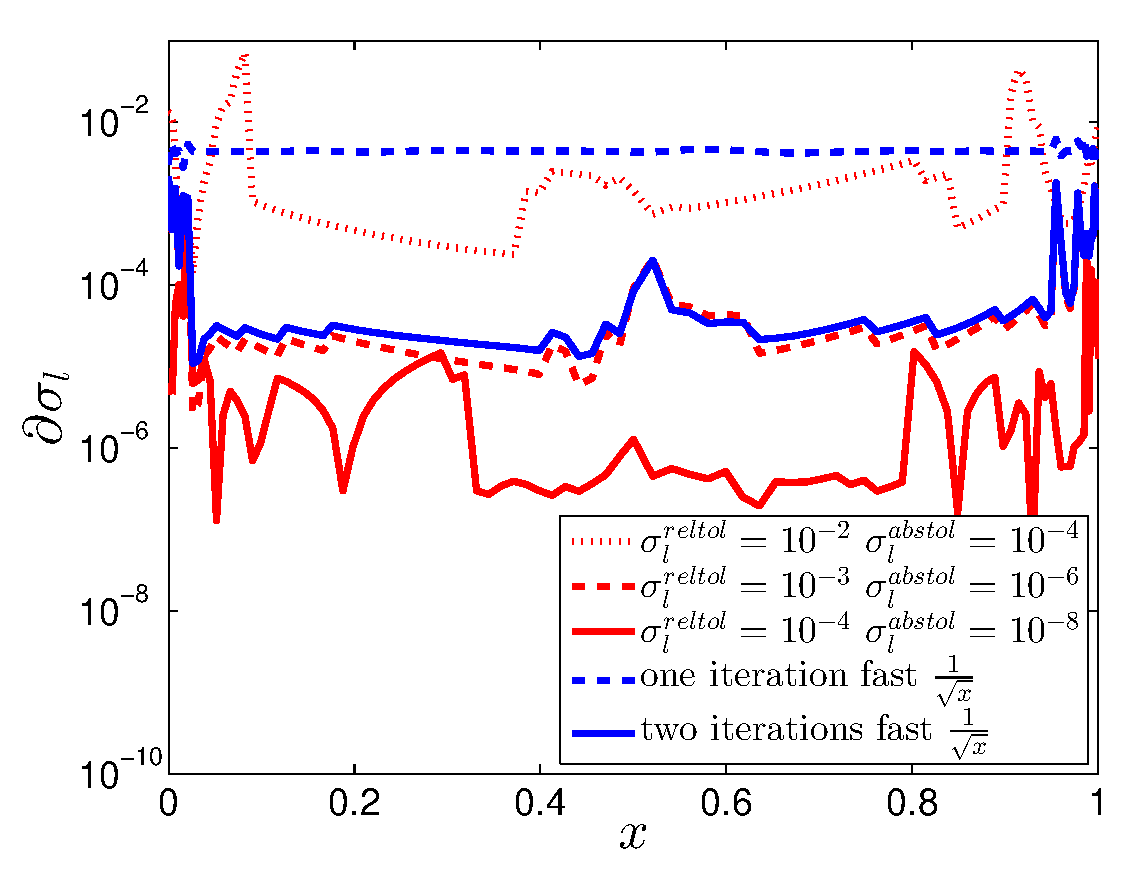
\includegraphics[scale=0.6]{sigma_accs} 

\protect\caption{Relative discrepancies in $\sigma_{l}$, depending on the desired
accuracies. The alternative calculations with fast $\frac{1}{\sqrt{x}}$
uses $\sigma_{l}^{reltol}=10^{-3}$ and $\sigma_{l}^{abstol}=10^{-6}$}


\label{sigma_tols}
\end{figure*}


\clearpage


\subsection{Pseudo elastic influence $\sigma_{l}$, in some sample geometries}

The method for resolving fracture visibility \ref{visibility_algorithm},
is rather complex and deserves a few extra tests to verify if the
produced results agree with expectations. On Figures \ref{sample_visibility1},
\ref{sample_visibility2} and \ref{sample_visibility3} some relatively
simple to analyze structures are presented. One can have a look on
the arrangements of edges, and deduce what the pattern of visibility
matrix would be. Consequently the output of algorithm \ref{visibility_algorithm}
can be check against these empirical expectations.

First lets have a look at Figure \ref{sample_visibility1}. Here six
cracks are placed in such a way that $e_{3},e_{4}$ are in the center,
and $e_{1},e_{2},e_{5},e_{6}$ are on the outer edges of a short array
of fractures. This placement makes $e_{3},e_{4}$ visible to all $e_{1},e_{2},e_{5},e_{6}$,
which can be confirmed by presented visibility pattern. Furthermore
the end tips of $e_{1},e_{2}$ are long enough extend beyond the shadow
of center fractures, are are visible to end tips of $e_{5},e_{6}$
respectively. The value of $\sigma_{l}$ for the middle $e_{3},e_{4}$
at $x=0$ is double of that for outer $e_{1},e_{2},e_{5},e_{6}$,
as the middle is influenced by two fractures, while outer segments
only by one fracture. As the pair $e_{1},e_{2}$ is the longest, the
end tips $x=1$ are furthermost away form the rest of $\sigma_{l}$
sources, thous the value of $\sigma_{l}$ is the lowest at these points.
However having a closer look at $\sigma_{l}$ for $e_{1},e_{2}$ one
can notice that the rate of change slightly decreases near the tip.,
which should be associated with these tips being also exposed to parts
of $e_{5},e_{6}$.

On the next Figure \ref{sample_visibility2}, a number of PKN segments
are connected to each other directly. The visibility matrix shows
only full squares, as all the fractures are fully visible to each
other, or not visible at all. The effect of $min(d^{3},1)$ in (\ref{sigma_formula})
on $\sigma_{l}$ can be well observed here. For the relatively long
$e_{1}$, the reduction of $\sigma_{l}$ occurs at relatively close
proximity of the crack tip $x=1$. The distribution of $\sigma_{l}$
is most affected for the shortest $e_{4}$. Whether this is a serious
issue or not, is a hard question to answer.

Finally Figure \ref{sample_visibility3} consist of a mixture of partially
and fully visible interconnected PKN cracks and pipes. Pipe segment
$e_{1}$, as expected is seen by all the other edges, with the exception
of $e_{5}$ and parts of $e_{7}$, which is well reflected in the
visibility matrix . The presence of $e_{4},e_{5}$ affects $\sigma_{l}$
for $e_{7}$ as a local maxima near $x\approx0.5$ can be observed.
Even in such a case of relatively small test scenario, much more observations
could be made. However as complex as the pattern of visibility matrix
and distribution of $\sigma_{l}$ might be, the generic formulation
for obtaining these presented in this work produces valid and consistent
results, which is an achievement in its own. Having verified the procedure
for this examples, it is reasonable to assume that other possible
arrangements of fractures will also be properly handled.

\begin{figure*}[t]
\centering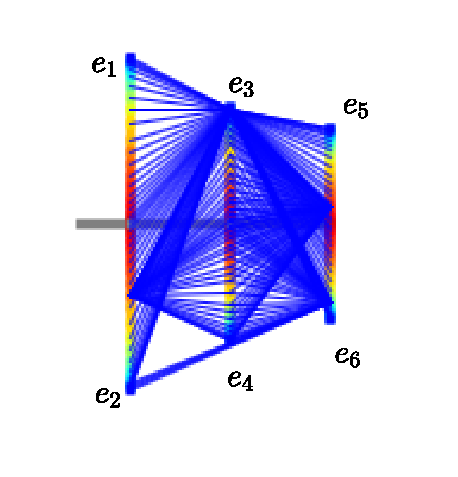
\includegraphics[scale=0.5]{vis1}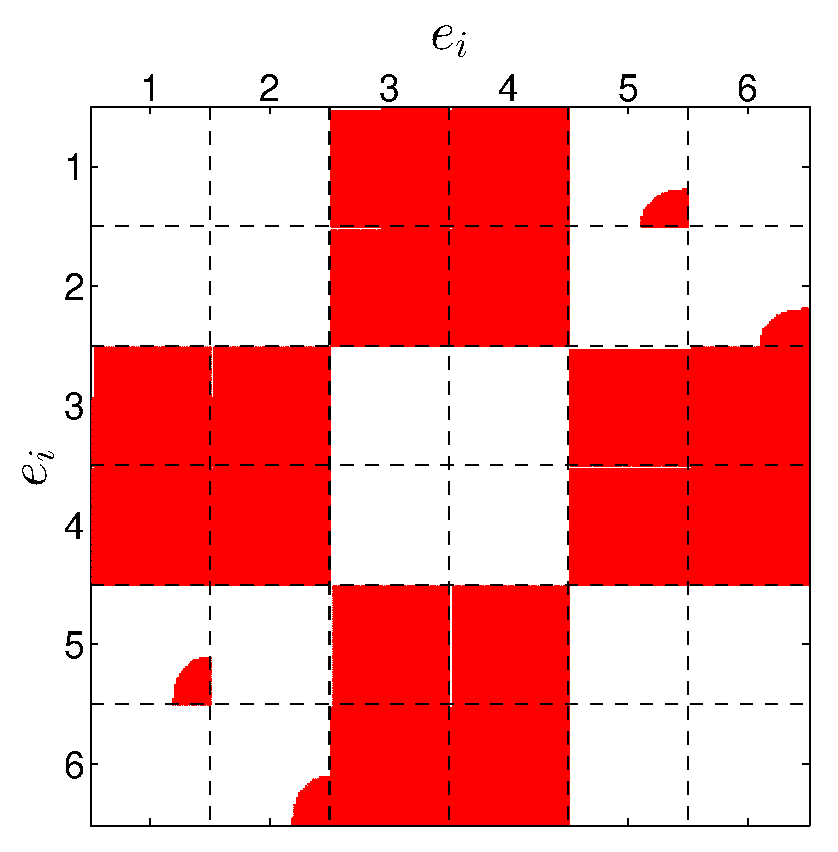
\includegraphics[scale=0.5]{vis1_mat} 

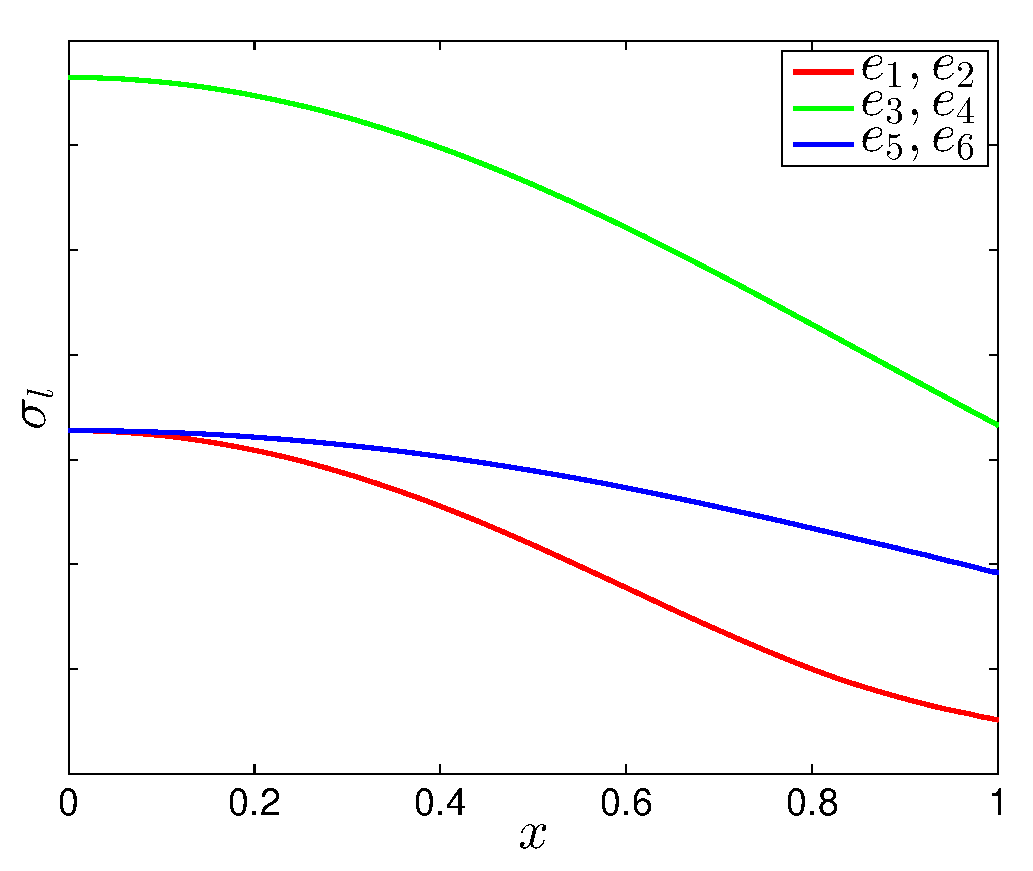
\includegraphics[scale=0.65]{vis1_sig} 

\protect\caption{Example visibility matrix and $\sigma_{l}$, array of PKN fractures
connected by solid pipes.}


\label{sample_visibility1}
\end{figure*}


\begin{figure*}[t]
\centering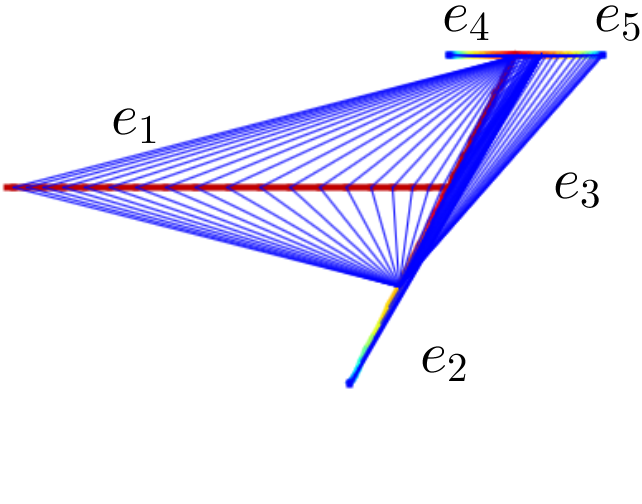
\includegraphics[scale=0.5]{vis2}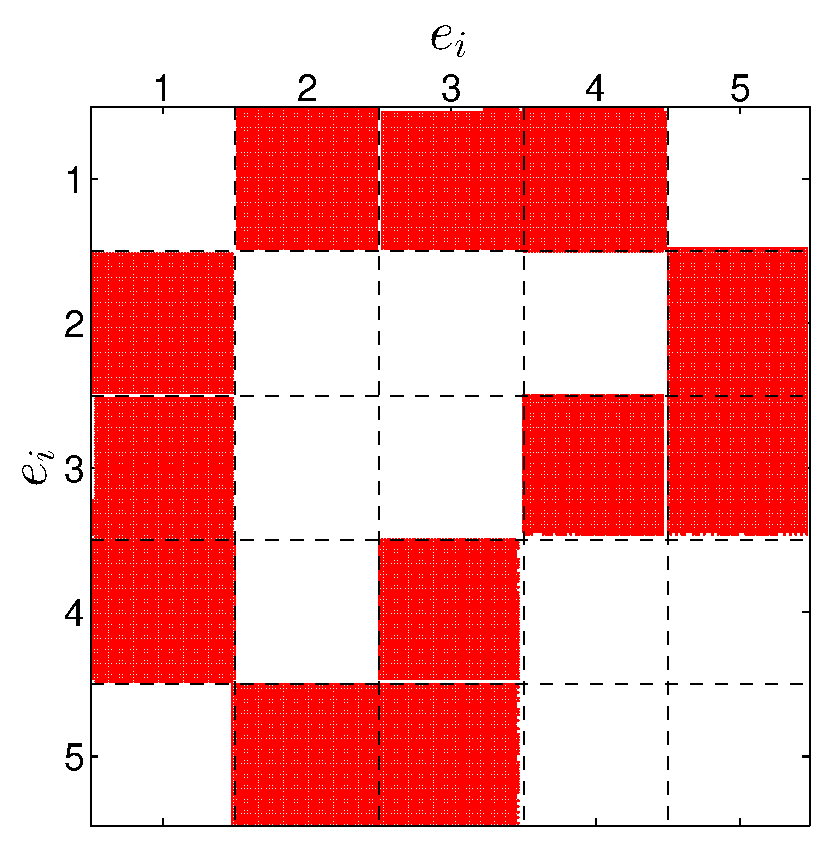
\includegraphics[scale=0.5]{vis2_mat} 

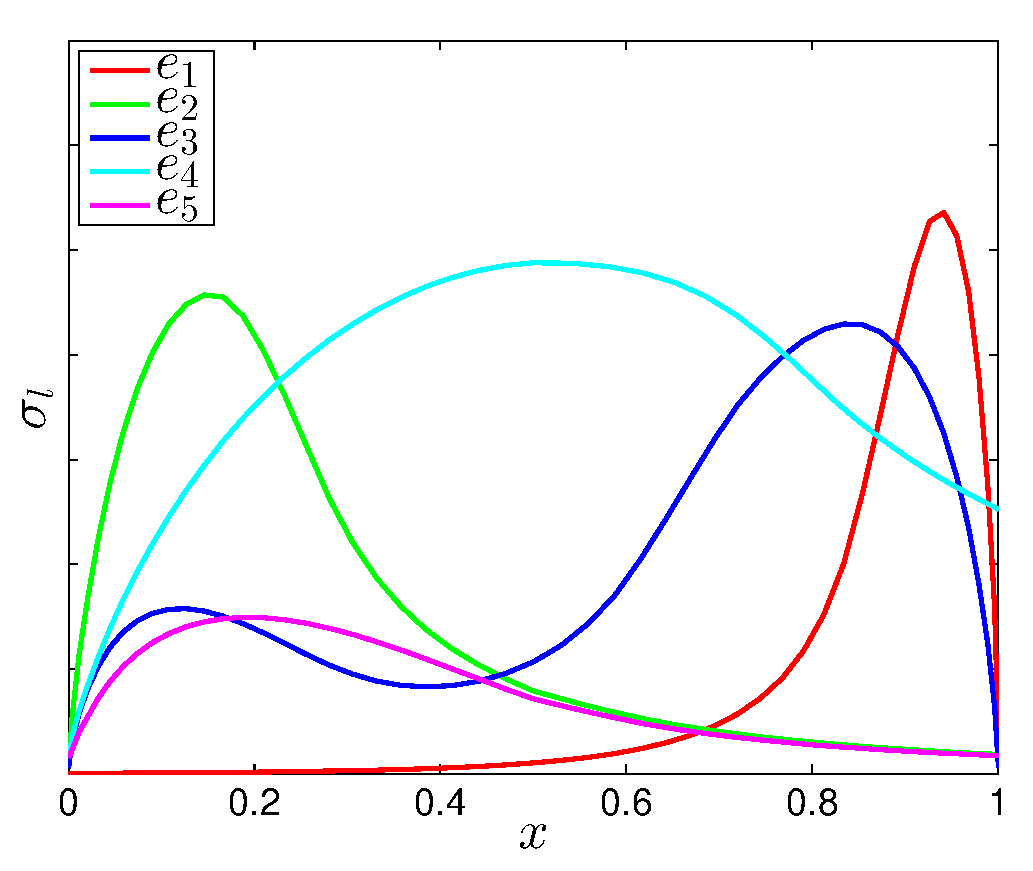
\includegraphics[scale=0.65]{vis2_sig} \label{sample_visibility2}

\protect\caption{Example visibility matrix and $\sigma_{l}$, a set of connected PKN
cracks and pipes.}
\end{figure*}
\begin{figure*}[t]
\centering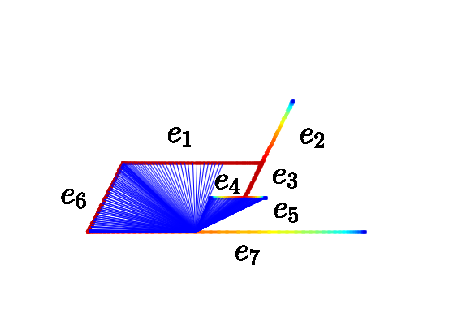
\includegraphics[scale=0.5]{vis3}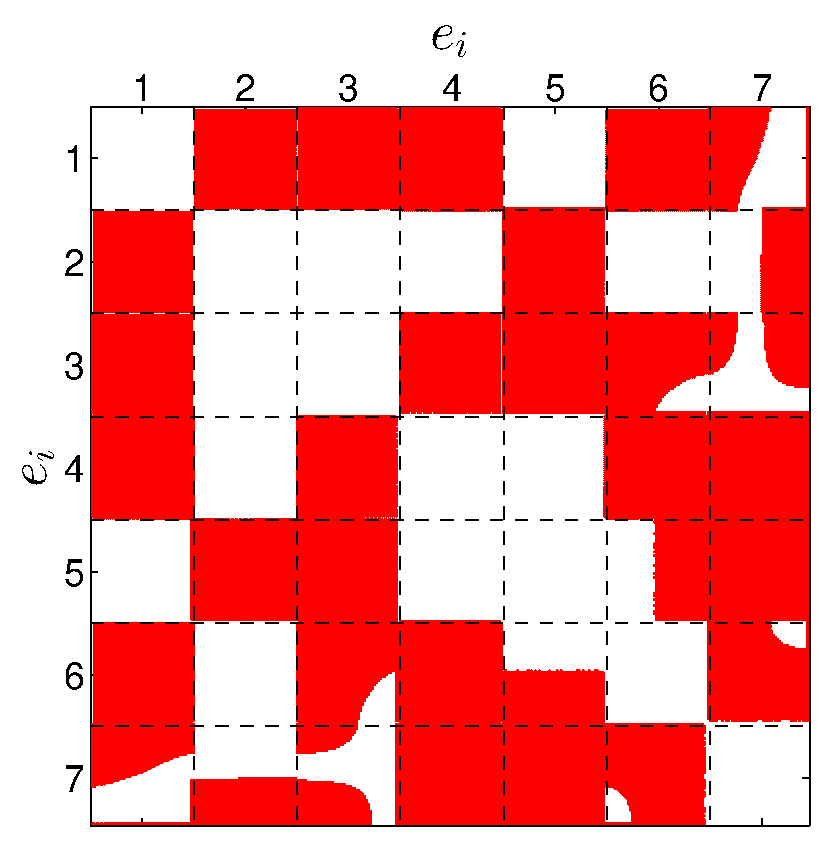
\includegraphics[scale=0.5]{vis3_mat} 

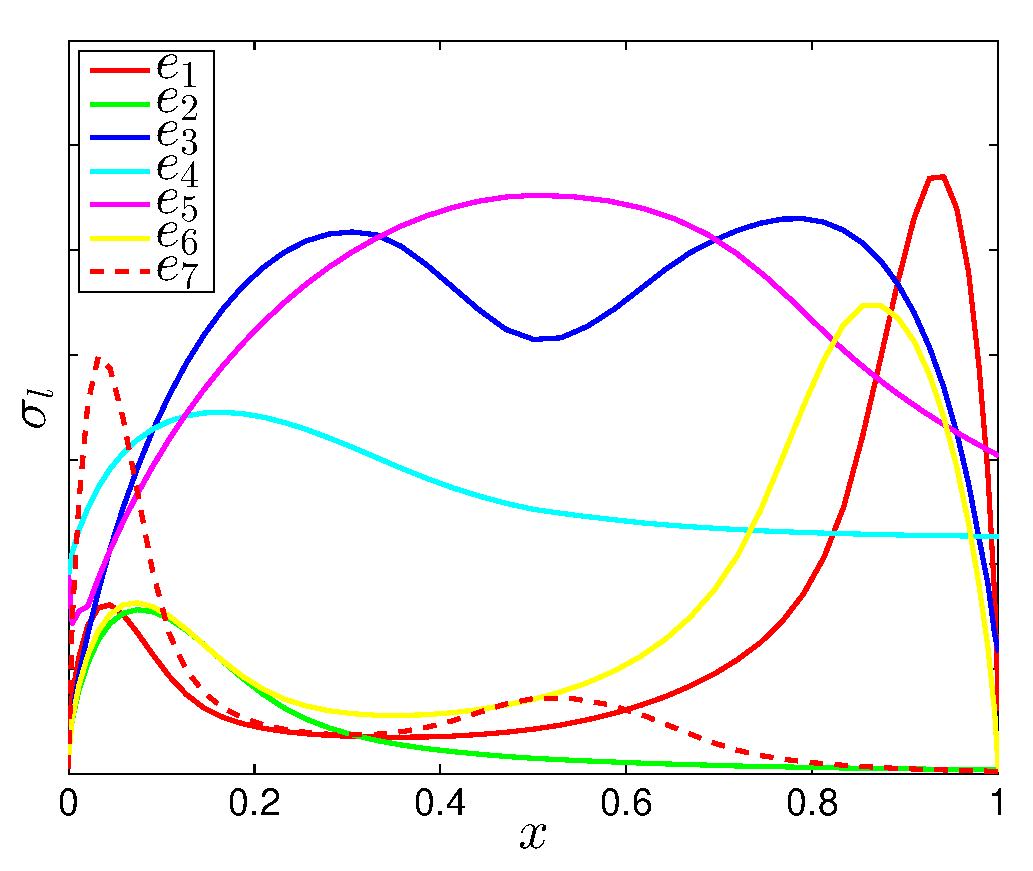
\includegraphics[scale=0.65]{vis3_sig} 

\protect\caption{Example visibility matrix and $\sigma_{l}$, a set of connected PKN
cracks and pipes with some partial visibilities.}


\label{sample_visibility3}
\end{figure*}


\clearpage


\subsection{Power input in an array of fractures}


\subsubsection{Uncoupled array}

In the work by Bunger \cite{Bunger} as mentioned before in section
{[}ref to elastic interactions again{]}, a test scenario was developed.
In this scenario a number $N_{fracture}$of double wing fractures
is placed in a parallel array at some area of fixed width $Z$. The
work was conducted on many radial, KGD and PKN model, and one of its
goals was to approximate the number of placed fractures that minimizes
power input required to maintain constant pump in rate over time.
That analytical work test can be reproduced for PKN model using numerical
methods introduced in this work. First lets write the spacing of fractures
$H$ and $q_{i}$ the individual pumping rate for each half fracture
wing:

\[
H=\frac{Z}{N_{fracture}},\quad q_{i}=\frac{q_{0}}{N_{fracture}}
\]


Which follow the test scenario proposed by Bunger. Thous in this case
flow is amused to disperse evenly to each fracture resulting in the
save value of pumping$q_{i}$ for each fracture. The total array power
input is approximated by summing:

fluid pressure $p_{fluid}$ at crack inlet, $x=0$, for each half
fracture in the array: 
\[
P(t)=\sum_{1}^{N_{fracture}}q_{i}p_{fluid}(t,0)
\]


This must be done with strict interpretation of elasticity approximation,
the stress must be set to be inversely proportional to$d^{3}$:

\begin{equation}
\sigma_{l}^{(j)}=\frac{gkw_{j}\Delta x_{j}L}{d^{3}}|(\hat{n_{j}}\cdot\hat{\sigma})(\hat{n_{i}}\cdot\hat{\sigma})|\label{sigma_formula_strict-1}
\end{equation}


Naturally one should expect slight variance in the obtained results,
as Bunger's tests have the same L and sigma for all fractures

Now lets make a more sophisticated test where $q_{i}$ is fixed and
the same for all connected fractures, but instead a \emph{solid pipe
segment} is used to connect all fractures in this array. Fractures
now will receive different ... zrobi\'{c} to p�\'{z}niej

\begin{figure}
\centering\includegraphics[scale=0.5]{\string"../Comparision with other works/power_arr_1\string".eps}

\centering\includegraphics[scale=0.5]{\string"../Comparision with other works/bunger_result\string".eps}\label{testvsbunger-1}

\protect\caption{Wst\k{e}pny wynik, jest minimum dla jakiej\'{s} ilo\'{s}ci, trzeba
przeliczy\'{n} z dok\l adnie tymi samymi k,E,$\mu$ itp. Wa\.{z}ne
\.{z}e generalnie to samo zachowanie}
\end{figure}



\subsubsection{Coupled array (to be done later when after some bugs in code are
fixed)}

\clearpage
\end{document}
